\documentclass{article}
\usepackage{amsmath,amssymb}
\usepackage{enumerate,mathtools}
\usepackage[letterpaper,margin=1in]{geometry}
\usepackage{hyperref}
\usepackage{tikz}
\usepackage{pgfplots}

% Theorems
\usepackage{amsthm}
\renewcommand\qedsymbol{$\blacksquare$}

\newtheorem{definition}{Definition}[section]
\newtheorem{example}{Example}[section]
\newtheorem{theorem}{Theorem}[section]
\newtheorem{corollary}[theorem]{Corollary}
\newtheorem{lemma}[theorem]{Lemma}


% Linear Algebra %

\setlength\unitlength{1mm}

\newcommand{\insertfig}[3]{
\begin{figure}[htbp]\begin{center}\begin{picture}(120,90)
\put(0,-5){\includegraphics[width=12cm,height=9cm,clip=]{#1.eps}}\end{picture}\end{center}
\caption{#2}\label{#3}\end{figure}}

\newcommand{\insertxfig}[4]{
\begin{figure}[htbp]
\begin{center}
\leavevmode \centerline{\resizebox{#4\textwidth}{!}{\input
#1.pstex_t}}
%\vspace*{-0.2in}
\caption{#2} \label{#3}
\end{center}
\end{figure}}

\long\def\comment#1{}

\newcommand\norm[1]{\left\lVert#1\right\rVert}
\DeclareMathOperator*{\argmin}{arg\,min}
\DeclareMathOperator*{\argmax}{arg\,max}
% bb font symbols

\newfont{\bbb}{msbm10 scaled 700}
\newcommand{\CCC}{\mbox{\bbb C}}

\newfont{\bbf}{msbm10 scaled 1100}
\newcommand{\CC}{\mbox{\bbf C}}
\newcommand{\PP}{\mbox{\bbf P}}
\newcommand{\RR}{\mbox{\bbf R}}
\newcommand{\QQ}{\mbox{\bbf Q}}
\newcommand{\ZZ}{\mbox{\bbf Z}}
\renewcommand{\SS}{\mbox{\bbf S}}
\newcommand{\FF}{\mbox{\bbf F}}
\newcommand{\GG}{\mbox{\bbf G}}
\newcommand{\EE}{\mbox{\bbf E}}
\newcommand{\NN}{\mbox{\bbf N}}
\newcommand{\KK}{\mbox{\bbf K}}

% Vectors

\renewcommand{\aa}{{\bf a}}
\newcommand{\bb}{{\bf b}}
\newcommand{\cc}{{\bf c}}
\newcommand{\dd}{{\bf d}}
\newcommand{\ee}{{\bf e}}
\newcommand{\ff}{{\bf f}}
\renewcommand{\gg}{{\bf g}}
\newcommand{\hh}{{\bf h}}
\newcommand{\ii}{{\bf i}}
\newcommand{\jj}{{\bf j}}
\newcommand{\kk}{{\bf k}}
\renewcommand{\ll}{{\bf l}}
\newcommand{\mm}{{\bf m}}
\newcommand{\nn}{{\bf n}}
\newcommand{\oo}{{\bf o}}
\newcommand{\pp}{{\bf p}}
\newcommand{\qq}{{\bf q}}
\newcommand{\rr}{{\bf r}}
\renewcommand{\ss}{{\bf s}}
\renewcommand{\tt}{{\bf t}}
\newcommand{\uu}{{\bf u}}
\newcommand{\ww}{{\bf w}}
\newcommand{\vv}{{\bf v}}
\newcommand{\xx}{{\bf x}}
\newcommand{\yy}{{\bf y}}
\newcommand{\zz}{{\bf z}}
\newcommand{\0}{{\bf 0}}
\newcommand{\1}{{\bf 1}}

% Matrices

\newcommand{\Ab}{{\bf A}}
\newcommand{\Bb}{{\bf B}}
\newcommand{\Cb}{{\bf C}}
\newcommand{\Db}{{\bf D}}
\newcommand{\Eb}{{\bf E}}
\newcommand{\Fb}{{\bf F}}
\newcommand{\Gb}{{\bf G}}
\newcommand{\Hb}{{\bf H}}
\newcommand{\Ib}{{\bf I}}
\newcommand{\Jb}{{\bf J}}
\newcommand{\Kb}{{\bf K}}
\newcommand{\Lb}{{\bf L}}
\newcommand{\Mb}{{\bf M}}
\newcommand{\Nb}{{\bf N}}
\newcommand{\Ob}{{\bf O}}
\newcommand{\Pb}{{\bf P}}
\newcommand{\Qb}{{\bf Q}}
\newcommand{\Rb}{{\bf R}}
\newcommand{\Sb}{{\bf S}}
\newcommand{\Tb}{{\bf T}}
\newcommand{\Ub}{{\bf U}}
\newcommand{\Wb}{{\bf W}}
\newcommand{\Vb}{{\bf V}}
\newcommand{\Xb}{{\bf X}}
\newcommand{\Yb}{{\bf Y}}
\newcommand{\Zb}{{\bf Z}}

% Calligraphic

\newcommand{\Ac}{{\cal A}}
\newcommand{\Bc}{{\cal B}}
\newcommand{\Cc}{{\cal C}}
\newcommand{\Dc}{{\cal D}}
\newcommand{\Ec}{{\cal E}}
\newcommand{\Fc}{{\cal F}}
\newcommand{\Gc}{{\cal G}}
\newcommand{\Hc}{{\cal H}}
\newcommand{\Ic}{{\cal I}}
\newcommand{\Jc}{{\cal J}}
\newcommand{\Kc}{{\cal K}}
\newcommand{\Lc}{{\cal L}}
\newcommand{\Mc}{{\cal M}}
\newcommand{\Nc}{{\cal N}}
\newcommand{\Oc}{{\cal O}}
\newcommand{\Pc}{{\cal P}}
\newcommand{\Qc}{{\cal Q}}
\newcommand{\Rc}{{\cal R}}
\newcommand{\Sc}{{\cal S}}
\newcommand{\Tc}{{\cal T}}
\newcommand{\Uc}{{\cal U}}
\newcommand{\Wc}{{\cal W}}
\newcommand{\Vc}{{\cal V}}
\newcommand{\Xc}{{\cal X}}
\newcommand{\Yc}{{\cal Y}}
\newcommand{\Zc}{{\cal Z}}

% Bold greek letters

\newcommand{\alphab}{\hbox{\boldmath$\alpha$}}
\newcommand{\betab}{\hbox{\boldmath$\beta$}}
\newcommand{\gammab}{\hbox{\boldmath$\gamma$}}
\newcommand{\deltab}{\hbox{\boldmath$\delta$}}
\newcommand{\etab}{\hbox{\boldmath$\eta$}}
\newcommand{\lambdab}{\hbox{\boldmath$\lambda$}}
\newcommand{\epsilonb}{\hbox{\boldmath$\epsilon$}}
\newcommand{\nub}{\hbox{\boldmath$\nu$}}
\newcommand{\mub}{\hbox{\boldmath$\mu$}}
\newcommand{\zetab}{\hbox{\boldmath$\zeta$}}
\newcommand{\phib}{\hbox{\boldmath$\phi$}}
\newcommand{\psib}{\hbox{\boldmath$\psi$}}
\newcommand{\thetab}{\hbox{\boldmath$\theta$}}
\newcommand{\taub}{\hbox{\boldmath$\tau$}}
\newcommand{\omegab}{\hbox{\boldmath$\omega$}}
\newcommand{\xib}{\hbox{\boldmath$\xi$}}
\newcommand{\sigmab}{\hbox{\boldmath$\sigma$}}
\newcommand{\pib}{\hbox{\boldmath$\pi$}}
\newcommand{\rhob}{\hbox{\boldmath$\rho$}}

\newcommand{\Gammab}{\hbox{\boldmath$\Gamma$}}
\newcommand{\Lambdab}{\hbox{\boldmath$\Lambda$}}
\newcommand{\Deltab}{\hbox{\boldmath$\Delta$}}
\newcommand{\Sigmab}{\hbox{\boldmath$\Sigma$}}
\newcommand{\Phib}{\hbox{\boldmath$\Phi$}}
\newcommand{\Pib}{\hbox{\boldmath$\Pi$}}
\newcommand{\Psib}{\hbox{\boldmath$\Psi$}}
\newcommand{\Thetab}{\hbox{\boldmath$\Theta$}}
\newcommand{\Omegab}{\hbox{\boldmath$\Omega$}}
\newcommand{\Xib}{\hbox{\boldmath$\Xi$}}


% mixed symbols

\newcommand{\sinc}{{\hbox{sinc}}}
\newcommand{\diag}{{\hbox{diag}}}
\renewcommand{\det}{{\hbox{det}}}
\newcommand{\trace}{{\hbox{tr}}}
\newcommand{\tr}{\trace}
\newcommand{\sign}{{\hbox{sign}}}
\renewcommand{\arg}{{\hbox{arg}}}
\newcommand{\var}{{\hbox{var}}}
\newcommand{\cov}{{\hbox{cov}}}
\renewcommand{\Re}{{\rm Re}}
\renewcommand{\Im}{{\rm Im}}
\newcommand{\eqdef}{\stackrel{\Delta}{=}}
\newcommand{\defines}{{\,\,\stackrel{\scriptscriptstyle \bigtriangleup}{=}\,\,}}
\newcommand{\<}{\left\langle}
\renewcommand{\>}{\right\rangle}
\newcommand{\Psf}{{\sf P}}
\newcommand{\T}{\top}
\newcommand{\m}[1]{\begin{bmatrix} #1 \end{bmatrix}}


\newcommand*{\horzbar}{\rule[.5ex]{2.5ex}{0.5pt}}
\newcommand{\rank}{\mathrm{rank}}

\setlength{\parindent}{0pt}

\begin{document}

\begin{center}
  \Large\textbf{Linear Algebra Review}\\
  \large\textit{Conner DiPaolo}
\end{center}
\vspace*{1em}

\tableofcontents
\vspace{1em}

This is an adaptation of Stanford's CS229 \textit{Linear Algebra Review and Reference}
\footnote{\url{http://cs229.stanford.edu/section/cs229-linalg.pdf}}, written by Zico Kolter
and updated by Chuong Do, and some extra material that will be helpful in the
course.\\

\textbf{To the Reader:} If you want a brief and \textit{very} comprehensive reference/resource
of anything Linear Algebra related (including a ton of matrix derivatives at the beginning)
check out the Matrix Cookbook \footnote{\url{https://www.math.uwaterloo.ca/~hwolkowi/matrixcookbook.pdf}}.
It has over 800 citations in the literature!

\section{Basics}

Linear Algebra allows us to interact with linear operators (or systems
of linear equations) in a more powerful manner than dealing with equations.
For example, consider the linear system
\begin{align*}
    x_1 + 2x_2 &= 5\\
    3x_1 + 4x_2 &= 1.
\end{align*}
This can be solved for $x_1$ and $x_2$ using substitution, but it is
convenient (for many reasons) to investigate this system more compactly,
as a matrix-vector product. Namely,
\[
    A\xx = \bb
\]
where
\[
    A = \m{1&2\\3&4} \quad\text{and}\quad \bb = \m{5\\1}.
\]
Here, $A$ is a \textit{matrix} and $\bb$ is a \textit{vector}. Matrices are
\textit{linear operators}. That is, they obey the following property, where
$A$ is a matrix in $\RR^{m\times n}$, $\xx$ and $\yy$ are vectors in $\RR^n$,
and $c$ and $d$ are scalars:
\[
    A(c\xx+d\yy) = cA\xx + dA\yy.
\]
Note that this implies that
\[
    A\0 = \0.
\]

\subsection{Notation}

\begin{enumerate}[-]
    \item We denote an $m\times n$ matrix of real numbers $A$ as $A\in\RR^{m\times n}$
        (``A is in R m by n'').
        Similarly, to declare a $m\times n$ matrix of complex numbers we say $B\in\CC^{m\times n}$.
    \item We denote a vector $\xx$ with $n$ real elements as $x\in\RR^n$. By convention, $\xx$
        is assumed to be a column vector (that is, equivalently, $\xx\in\RR^{n\times 1}$).
        If we want to represent a row vector, we use $\xx^\T$, where $\T$ is the transpose.
    \item The $i-$th element of a vector $\xx$ is denoted $x_i$.
    \item We denote the $i,j$-th element of a matrix $A$ as $a_{ij}$, $A_{ij}$, or
        $A_{i,j}$.
        \[
            A = \m{a_{11} & a_{12}&\dots&a_{1n} \\ a_{21} & a_{22} & \dots & a_{2n}\\ \vdots&\vdots&\ddots&\vdots\\a_{m1}&a_{m2}&\dots&a_{mn}}
        \]
    \item We denote the $j-$th column of $A$ as $A_{:,j}$.
    \item We denote the $i-$th row of $A$ as $A_{i,:}$.
    \item $\1$ is the vector of all ones. $\0$ is the vector of
        all zeroes. Size is dependent on context.
\end{enumerate}

\section{Matrix Multiplication}

From the intro section we have already seen a matrix-vector product $A\xx$. We will
now define vector-vector products (the inner and outer product) and matrix-matrix
products (which encapsulate matrix-vector products).\\

The product of two matrices $A\in\RR^{m\times n}$ and $B\in\RR^{n\times p}$ is
the matrix
\[
    C = AB\in\RR^{m\times p}
\]
where
\[
    C_{ij} = \sum_{k=1}^n A_{ik}B_{kj}.
\]

\subsection{Vector-Vector Products}

Let $\xx,\yy\in\RR^n$. Then the \textit{inner product} (sometimes referred as the
dot product but we won't use that terminology)
\[
    \langle \xx,\yy \rangle = \xx^\T\yy = \sum_{i=1}^n \xx_i\yy_i = ||\xx||_2||\yy||_2\cos\theta
\]
where $\theta$ is the angle between the vectors.
Note that $\langle \cdot, \cdot \rangle: (V,V) \mapsto \RR$ (``$\langle \cdot, \cdot
\rangle$ maps two elements of the vector space $V$ to $\RR$'') here is the standard definition of
the inner product for the vector space $V=\RR^n$. As we will see later in the
class, other inner products can be defined between vectors in $\RR^n$.\\

The \textit{outer product} between $\xx\in\RR^m$ and $\yy\in\RR^n$ as
\[
    \xx\yy^\T \in \RR^{m\times n},
\]
a matrix.
\[
    (\xx\yy^\T)_{ij} = \xx_i\yy_j.
\]
This will be useful when we talk about Principal Component Analysis and
Covariance.

\subsection{Matrix-Vector Products}

The matrix-vector product between $A\in\RR^{m\times n}$ and $\xx\in\RR^n$ is
the vector $\yy = A\xx \in \RR^m$. We can see from the formula for matrix-matrix
multiplication that
\[
    A\xx = \m{|&|& &|\\a_1&a_2&\dots&a_n\\|&|& &|}\m{x_1\\x_2\\\dots\\x_n} = x_1\m{|\\a_1\\|} + x_2\m{|\\a_2\\|} + \dots + x_n\m{|\\x_n\\|},
\]
a linear combination of the columns of $A$!

\subsection{Matrix-Matrix Multiplication}

Armed with this knowledge, we can see matrix-matrix multiplication between
$A\in\RR^{m\times n}$ and $B\in\RR^{n\times p}$ as

\[
    AB = \m{|&|& &|\\a_1&a_2&\dots&a_n\\|&|& &|}\m{\horzbar&b_1^T&\horzbar\\\horzbar&b_2^T&\horzbar\\&\vdots&\\\horzbar&b_n^T&\horzbar} = \sum_{i=1}^n a_ib_i^\T = \m{a_i^\T b_1&a_2^\T b_2&\dots&a_1^\T b_p\\a_2^\T b_1& a_2^\T b_2i& \dots& a_2^\T b_p\\ \vdots & \vdots & \ddots & \vdots\\ a_m^\T b_1 & a_m^\T b_2 & \hdots & a_m^\T b_p},
\]
either an arrangement of every possible inner product between the rows of $A$
and the columns of $B$, or a sum of outer products between the columns of $A$
and the rows of $B$.

\subsection{Properties of Matrix Multiplication}

\begin{enumerate}[-]
    \item Matrix multiplication is associative: $(AB)C = A(BC)$
    \item Matrix multiplication is distributive: $A(B+C) = AB + AC$
    \item Matrix multiplication is not commutative \textit{in general}:
        $AB \neq BA$ (in the vast majority of cases).
\end{enumerate}

\section{Operations and Properties}

Most of this should hopefully be review, but if you haven't seen complex matrix operations
before don't worry we won't use them much.

\subsection{The Identity Matrix and Diagonal Matrices}

The \textit{identity matrix}, denoted $I\in\RR^{n\times n}$, is a square matrix
with ones on the diagonal and zeros everywhere else:
\[
    I_{ij} = \begin{cases} 1 & \text{if $i=j$}\\
        0 & \text{otherwise.}
    \end{cases}
\]
For any $A\in\RR^{m\times n}$,
\[
    AI = A = IA.
\]
Intuitively, this means that as an operator the identity matrix maps every
vector to itself.\\

A \textit{diagonal matrix} is a matrix where all non-diagonal elements are 0.
This is denoted $D=\mathrm{diag}(d_1,d_2,\dots,d_n)$ where
\[
    D_{ij} = \begin{cases}
        d_i & \text{if $i=j$}\\
        0 & \text{otherwise.}
    \end{cases}
\]

\subsection{The Transpose: $A^\T$}

The \textit{transpose} of a matrix is where every row becomes a column. Given
$A\in\RR^{m\times n}$, the transpose of $A$, $A^\T\in\RR^{n\times m}$ is defined
as
\[
    (A^\T)_{ij} = A_{ji}.\\
\]

Here are some helpful properties (proofs are easily verifiable):
\begin{enumerate}[-]
\item $(A^\T)^\T = A$
\item $(AB)^\T = B^\T A^\T$
\item $(A+B)^\T = A^\T + B^\T$
\end{enumerate}

\subsection{Symmetric Matrices}

A matrix $S\in\RR^{n\times n}$ is \textit{symmetric} if and only if
$S = S^\T$. For any $A\in\RR^{n\times n}$, $A+A^\T$ and $A^\T A$
are both symmetric. This is easily verified from the above properties.
We denote the set of symmetric matrices in $\RR^{n\times n}$ as $\SS^n$.
As we will see, symmetric matrices are often nice to work with.

\subsection{The Conjugate Transpose: $A^*$}

For complex matrices $A\in\CC^{m\times n}$, the conjugate transpose of
$A$, said ``$A$ Hermitian'' is denoted as $A^* = \overline{A^\T}$.
That is,
\[
    (A^*)_{ij} = \overline{A}_{ji}.
\]
For example,
\[
    \m{1+2\ii & 3\ii\\ 1 & 2-\ii}^* = \m{1-2\ii&1\\-3\ii&2+\ii}
\]

\subsection{Hermitian Matrices}

A matrix is Hermitian if $A = A^*$. This is a generalization of symmetric
matrices from real to complex matrices.

\subsection{The Trace $\tr(A)$}

The trace of a square matrix $A\in\RR^{n\times n}$ is the sum of the diagonal
elements:
\[
    \tr A = \tr(A) = \sum_{i=1}^n A_{ii}.
\]
Here are some useful properties:
\begin{enumerate}[-]
\item For $A\in\RR^{n\times n}$, $\tr A = \tr A^\T$
\item For $A,B\in\RR^{n\times n}$, $\tr(A+B) = \tr A + \tr B$
\item For $A,B$ such that $AB$ is square, $\tr AB = \tr BA$
\item For $A,B,C$ such that $ABC$ is square, $\tr ABC = \tr BCA
    = \tr CAB$, and this can be extended to more matrices.
\end{enumerate}

(from CS229) Here's a proof of the fourth property:
\begin{align*}
    \tr AB &= \sum_{i=1}^m(AB)_{ii}\\
    &= \sum_{i=1}^m\sum_{j=1} A_{ij}B_{ij}\\
    &= \sum_{j=1}^n\sum_{i=1}^m B_{ij}A_{ij} = \sum_{j=1}^n (BA)_{ii}\\
    &= \tr BA,
\end{align*}
as desired.

A very useful property is that the trace of a matrix is the sum
of the eigenvalues of that matrix, as we will see.

\subsection{Norms}

A \textit{norm} of a vector $||\xx||$ is to an approximation a measure of
length of $\xx$. We define the $\ell-p$ norm as
\[
    ||\xx||_p = \left( \sum_{i=1}^n x_i^p \right)^{1/p}.
\]
The \textit{distance} between a two vectors is in an $\ell-p$ space
is $||\xx-\yy||_p$. Euclidean distance, $||\xx-\yy||_2$ is what we normally
consider as `distance'.

There are really 4 cases of the $\ell-p$ norm that we might encounter:
\begin{enumerate}[-]
    \item $||\xx||_0 = $(the number of non-zero elements of $\xx$)
    \item $||\xx||_1 = \sum |\xx_i|$. We call $||\xx-\yy||_1$ the \textit{Manhatten Distance}
        between $\xx$ and $\yy$ because it treats walking between coordinates in
        $\RR^n$ as walking on perpendicular streets. This is opposed to Euclidean Distance
        where you can walk in a strait line from point to point.
    \item $||\xx||_2 = \sqrt{\sum\xx_i}$ is the Euclidean Norm. This is what we normally
        consider as the `length' of a vector.
    \item $||\xx||_\infty = \max_i |x_i|$.
\end{enumerate}
We will encounter $\ell-p$ norms \textit{a lot} in our studies. Specifically, we can
improve the robustness of many algorithms to outliers by constraining the norm
of some parameter in our optimization. Infinitely many other norms can be defined,
however. A norm is \textit{any} function $f : \RR^n \mapsto \RR$ that satisfies 4
properties:
\begin{enumerate}
\item For all $\xx\in\RR^n$, $f(\xx)\geq 0$ \hfill (non-negativity)
\item $f(\xx)=0$ if and only if $\xx=\0$ \hfill (definiteness)
\item For all $\xx\in\RR^n$ and $t\in\RR$, $f(t\xx) = |t|f(\xx)$ \hfill (homogeneity)
\item For all $\xx,\yy\in\RR^n$, $f(\xx+\yy) \leq f(\xx) + f(\yy)$ \hfill (triangle inequality)\\
\end{enumerate}

Norms can be extended to matrices too, as we will encounter. Here are
a few, where $A\in\RR^{m\times n}$:
\begin{enumerate}
    \item $||A||_F = \sqrt{\sum_{i=1}^m\sum_{j=1}^n A_{ij}^2} = \sqrt{\tr(A^\T A)}$ is the Frobenius Norm of $A$.
    \item $||A||_* = \tr(\sqrt{A^* A}) = \sum_{i=1}^{\min\{m,n\}}\sigma_i = $(sum of the singular values of $A$) is the Nuclear Norm
    \item $||A||_{\mathrm{max}} = \max_{ij}|A_{ij}|$
    \item $||A||_2 = \sqrt{\lambda_{max}(A^* A)} = \sigma_{max}(A)$ is the Spectral Norm.
\end{enumerate}

\subsection{Linear Independence, Span and Rank}

A \textit{linear combination} of the vectors $\xx_1,\xx_2,\dots,\xx_n$ is a sum
of scalar multiples of each of the vectors. That is, for $\alpha_i\in\RR$,
\[
    \alpha_1\xx_1 + \alpha_2\xx_2 + \dots + \alpha_n\xx_n
\]
is a linear combination of those vectors, for any $\alpha_i$.\\

The \textit{span} of a set of vectors $X = \{\xx_1,\xx_2,\dots,\xx_n\} \subset \RR^m$
is every possible linear combination of $X$:
\[
    \mathrm{span}\{\xx_1,\xx_2,\dots,\xx_n\} = \alpha_1\xx_1 + \alpha_2\xx_2 + \dots + \alpha_n\xx_n
\]
for any $\alpha_1,\alpha_2,\dots,\alpha_n\in\RR$.\\

A set of vectors $\{\xx_1,\xx_2,\dots,\xx_n\} \subset \RR^m$ is
\textit{linearly independent} if no vector can be represented as
a linear combination of the others. If some
\[
    \xx_i \in \mathrm{span}\{\xx_1,\xx_2,\dots, \xx_{i-1}, \xx_{i+1},\dots,\xx_n\},
\]
the vectors are said to be \textit{linearly dependent}. As an example,
the vectors
\[
    \xx_1 = \m{1\\1\\1} \qquad \xx_2 = \m{1\\2\\3} \qquad \xx_3 = \m{0\\1\\2}
\]
are linearly dependent because $\xx_3 = \xx_2-\xx_1$.\\

The \textit{rank} of a matrix $A\in\RR^{m\times n}$ is cardinality (size) of the largest set of
columns in $A$ that are linearly independent (this is also called the \textit{column rank} of $A$).
Coincidentally, this is also the cardinality of the largest set of \textit{rows} of $A$ that are 
linearly independent (this is also called the \textit{row rank} of $A$). Here are some helpful
properties of rank:
\begin{enumerate}
\item For $A\in\RR^{m\times n}$, $\rank(A)\leq\min(m,n)$. If $\rank(A)=\min(m,n)$, then $A$
    is said to be \textit{full rank}.
\item For $A\in\RR^{m\times n}$, $\rank(A) = \rank(A^\T)$.
\item For $A\in\RR^{m\times n}$, $B\in\RR^{n\times p}$, $\rank(AB)\leq \min(\rank(A),\rank(B))$.
\item For $A,B\in\RR^{m\times n}$, $\rank(A+B)\leq \rank(A) + \rank(B)$.
\end{enumerate}

\subsection{The Inverse $A^{-1}$}

The \textit{inverse} of a matrix $A\in\RR^{n\times n}$, denoted $A^{-1}$, is the unique matrix
such that
\[
    A^{-1}A = I = AA^{-1}.
\]
If we think of $A$ as a linear map from vectors $V$ in $\RR^n$ to different vectors $W$ in $\RR^n$
such that $A : V \mapsto W$, the inverse $A^{-1}$ is the linear map (matrix) that maps vectors in
$W$ back to $V$ such that $A^{-1}: W \mapsto V$. Then $AA^{-1}:V\mapsto W\mapsto V = I$.
Note that this is an abuse of notation because
$V=W$ and the $\mapsto$ does not imply a bijective mapping, but nevertheless it should convey the
idea more intuitively.\\

Using this intuition, it should be clear that a matrix $A\in\RR^{m\times n}$, which maps $A: \RR^n
\mapsto \RR^m$ can not be invertible if $m\neq n$ because (without loss of generality suppose $m < n$)
then you are effectively `losing information' by projecting all of $\RR^n$ into a smaller space which
you cannot recover.\\

To that end, a matrix $A\in\RR^{n\times n}$ is invertible if and only if $\rank(A) = n$. A matrix that
is non-invertible is called \textit{singular}. Here are some helpful properties:
\begin{enumerate}
\item $(A^{-1})^{-1} = A$
\item $(AB)^{-1} = B^{-1}A^{-1}$
\item $(A^{-1})^\T = (A^\T)^{-1}$. We often denote $(A^{-1})^\T$ as $A^{-\T}$ because
    of this fact.\\
\end{enumerate}

Given a linear system $A\xx=\bb$, if $A$ is invertible we can multiply on
the left by $A^{-1}$, giving
\[
    A^{-1}A\xx = I\xx = \xx = A^{-1}\bb,
\]
a closed form for $\xx$. For the love of all that is holy, however, \textit{please} do
not solve systems numerically by calculating the inverse of any matrices!
\footnote{at the very least instead of $A^{-1}\bb$ (\texttt{pinv(A)*b} Matlab or Julia) use $A\setminus\bb$
(\texttt{A$\backslash$b} in Matlab or Julia).} Computing the inverse in general
has numerical precision issues when done on a computer.

\subsection{Orthogonal Matrices}

Two vectors $\xx,\xx\in\RR^n$ are orthogonal if $\xx^\T\yy = 0$. A vector $\xx$ is normalized (that is,
$\xx$ is a unit vector) if $||\xx||_2 = 1$. A square matrix $Q\in\RR^{n\times n}$ is \textit{orthogonal}
if all of it's columns are orthogonal to each other and are normalized (in this case, we say that
the collection of column vectors are \textit{orthonormal}). Thus for any orthogonal $Q$,
\[
    Q^\T Q = I = QQ^\T,
\]
so $Q^{-1} = Q^\T$. We have another nice property as well, where for any vector $\xx\in\RR^{n}$
and orthogonal $Q\in\RR^{n\times n}$,
\[
    ||Q\xx||_2 = ||\xx||_2
\]
directly from the linear-combination-of-columns definition of matrix-vector multiplication.

\subsection{Unitary Matrices}

Just like Hermitian matrices extend symmetry to complex matrices, a unitary matrix
$U\in\CC^{n\times n}$ has columns $\{\uu_1,\uu_2,\dots,\uu_n\}$ such that
\[
    \uu_i^\T\overline\uu_j = \begin{cases}
        1 & \text{if $i=j$}\\
        0 & \text{otherwise}
    \end{cases}
\]
Similarly, for any unitary $U$, $U^{-1} = U^*$.

\subsection{Columnspace and Nullspace of a Matrix}

Given $A\in\RR^{m\times n}$, the columnspace (sometimes
called the range) of $A$ is
\[
    \mathrm{col}(A) = \left\{A\xx : \xx\in\RR^n\right\} \subseteq \RR^m = \mathrm{span}\{A_{:,1}, \dots, A_{:,n}\}.
\]
This can be thought of as the output of the linear operator
the matrix represents, given any possible input. If $A$ is
square and has full rank, then $\mathrm{col}(A) = \RR^n$.\\

The nullspace of $A$ is the set
\[
    \mathrm{null}(A) = \left\{ \xx : A\xx = \0,\quad \xx\in\RR^n \right\}.
\]
interestingly enough, the Rank-Nullity Theorem states that
\[
    \mathrm{dim}(\mathrm{null}(A)) + \mathrm{dim}(\mathrm{col}(A)) = n.
\]

\subsection{Projections}

Suppose, given a matrix $A\in\RR^{m\times n}$ and a vector $\yy\in\RR^n$,
we want to find the closest vector $\xx\in\RR^n$ within the columnspace
of $A$. That is,
\[
    \mathrm{proj}_A \yy = P\yy = \xx = \argmin_{\xx\in\mathrm{col}(A)} ||\xx-\yy||_2.
\]
This is the \textit{projection} of $\yy$ onto $A$. The matrix $P$ that projects
any input vector onto the columnspace of $A$. It can be shown that
\[
    P = A(A^\T A)^{-1}A^\T.
\]
As we will see this looks awfully familiar to the least-squares closed-form
solution (and for good reason)!

\subsection{The Determinant}

The determinant of a square matrix $A\in\RR^{n\times n}$ is a function
$\det: \RR^{n\times n} \mapsto \RR$ often denoted $|A|$. Geometrically,
it corresponds to the area of the parallelogram (or parallelotope in
$n$ dimensions) given by the columns of $A$. For example, the matrix
\[
    A = \m{a&c\\b&d}
\]
has determinant $|A| = ad-cb$ (take this as a definition for the $2\times2$
case). Visually we can see the following:
\begin{center}
    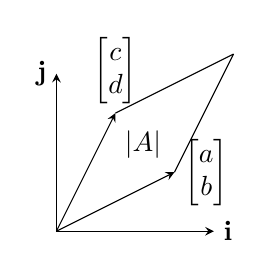
\begin{tikzpicture}
        \draw[-stealth] (0,0) -- (0,2) node[left] {$\mathbf{j}$};
        \draw[-stealth] (0,0) -- (2,0) node[right] {$\ii$};
        \draw[-stealth] (0,0) -- (1.5,0.75) node[right] {$\m{a\\b}$};
        \draw[-stealth] (0,0) -- (0.75,1.5) node[above] {$\m{c\\d}$};

        \draw (1.5,0.75) -- (2.25,2.25);
        \draw (0.75,1.5) -- (2.25,2.25);
        \draw (1.1,1.1) node {$|A|$};
    \end{tikzpicture}
\end{center}

Algebraically, we define the $(i,j)$ minor of $A$, $A_{\backslash i, \backslash j}$
as the matrix resulting from removing row $i$ and column $j$ from $A$. Then the
determinant becomes
\begin{align*}
    |A| &= \sum_{i=1}^n (-1)^{i+j}|A_{\backslash i,\backslash j}| \hfill \text{(for any $j\in 1,\dots,n$)}\\
        &= \sum_{j=1}^n (-1)^{i+j}|A_{\backslash i,\backslash j}| \hfill \text{(for any $i\in 1,\dots,n$)}\\
\end{align*}
The abjoint of $A\in\RR^{n\times n}$ is
\[
    \mathrm{adj}(A)_{ij} = (-1)^{i+j}|A_{\backslash i,\backslash j}|
\]
(note the switch of indices $A_{\backslash i,\backslash j}$). It can be shown that if $A$ is invertible
then
\[
    A^{-1} = \frac{1}{|A|}\mathrm{adj}(A).
\]
Never use this to compute the inverse, though, because computing the determinant takes
$n!$ time.\\

Here are some nice properties of the determinant:
\begin{enumerate}
    \item $|A|=0$ if and only if $A$ is singular.
    \item $|A|=|A^\T|$
    \item $|AB|=|A||B|$ if $A,B\in\RR^{n\times n}$
    \item if $A$ is invertible $|A^{-1}| = 1/|A|$.
\end{enumerate}

\subsection{Quadratic Forms and Positive Semidefinite Matrices}

This is a pretty important concept to know about. Given a square matrix $A\in\RR^{n\times n}$
and a vector $\xx\in\RR^n$, the scalar $\xx^\T A\xx$ is called a
\textit{quadratic form}. We have the following definitions (where we
always assume $\xx \neq \0$):
\begin{enumerate}[(a)]
    \item A symmetric matrix $A\in\SS^n$ is \textbf{positive definite}
        if for any $\xx\in\RR^n$, $\xx^\T A\xx > 0$. This is written
        $A \succ 0$, and the set of positive definite matrices is
        usually denoted $\SS_{++}^n$.
    \item A symmetric matrix $A\in\SS^n$ is \textbf{positive semidefinite}
        if for any $\xx\in\RR^n$, $\xx^\T A\xx \geq 0$. This is written
        $A \succeq 0$, and the set of positive semidefinite matrices is
        usually denoted $\SS_{+}^n$.
    \item A symmetric matrix $A\in\SS^n$ is \textbf{negative definite}
        if for any $\xx\in\RR^n$, $\xx^\T A\xx < 0$. This is written
        $A \prec 0$.
    \item A symmetric matrix $A\in\SS^n$ is \textbf{negative semidefinite}
        if for any $\xx\in\RR^n$, $\xx^\T A\xx \leq 0$. This is written
        $A \preceq 0$.
\end{enumerate}

We will see eigenvalues later, but $\xx^\T A \xx > 0$ iff all $\lambda_i > 0$,
and $\xx^\T A\xx \geq 0$ iff all $\lambda_i \geq 0$, etc.\\

The matrix $A^\T A$ is always positive semidefinite. if $A$ is full rank, $A^\T A$
is always positive definite.

\subsection{Eigenvalues and Eigenvectors: $A\xx = \lambda \xx$}

Given $A\in\RR^{n\times n}$ we say $\lambda\in\CC$ is an \textit{eigenvalue} of
$A$ and $\xx\in\CC^n$ is a corresponding \textit{eigenvector} of $A$ if
\[
    A\xx = \lambda \xx,\quad \xx \neq \0.
\]
This implies that
\begin{align*}
    A\xx &= \lambda I \xx\\
    (A-\lambda I)\xx &= 0,\text{ so}\\
    \det(A-\lambda I) &= 0.
\end{align*}
This is a useful method to compute eigenvalues by hand, though it is not
the method used in Matlab, for example, because (for one) computing the
determinant takes $n!$ time. We call $\det(A-\lambda I)$ the \textit{characteristic
polynomial} of $A$. Here are some nice properties of eigenvalues:
\begin{enumerate}
    \item $\mathrm{tr}(A) = \sum_{i=1}^n \lambda_i$
    \item $|A| = \prod_{i=1}^n \lambda_i$
    \item $\rank (A) = $(the number of non-zero eigenvalues of $A$)
    \item If $A$ is invertible then $1/\lambda_i$ is an eigenvalue of
        $A^{-1}$ with the same corresponding eigenvector as $A$
    \item The eigenvalues of a diagonal matrix $D=\mathrm{diag}(d_1,\dots,d_n)$
        are just the diagonal entries $d_1,\dots,d_n$.
\end{enumerate}

We can write all eigenvector equations simultaneously as
\[
    AX = X\Lambda,
\]
so if we have $n$ linearly independent eigenvectors creating $X$,
$X$ is invertible, and right-multiplying by $X^{-1}$ we find
\[
    A = X\Lambda X^{-1}.
\]
This is called the \textit{eigendecomposition} of $A$, and if
possible $A$ is called \textit{diagonalizable}. This is the first
decomposition we will encounter, but we will see more soon.

\subsection{Eigenvalues and Eigenvectors of Symmetric Matrices}

Given $A\in\SS^n$ it can be shown that all eigenvalues of $A$ are
real and all corresponding eigenvectors are orthonormal. Using this,
we can show that the definiteness of a matrix can be determined only
from its eigenvalues. Suppose $A\in\SS^n = Q\Lambda Q^\T$. Then
\[
    \xx^\T A\xx = \xx^\T Q\Lambda Q^\T\xx = \yy^\T\Lambda\yy = \sum_{i=1}^n \lambda_i\yy_i^2.
\]
Thus if all $\lambda_i > 0$, $\xx^\T A\xx > 0$. This is trivially extended
to negative semidefiniteness, etc.

\section{Matrix Factorizations}

We have already seen the \textit{eigendecomposition} of a matrix $A$,
but this is not always available (we require $n$ linearly independent
eigenvectors). This decomposition helped us connect eigenvalues to
definiteness. We will see that there are other helpful decompositions
that apply to different (or all!) classes of matrices.

\subsection{Eigendecomposition: $A = X\Lambda X^{-1}$}

To recap, if a matrix $A\in\RR^{n\times n}$ has $n$ linearly independent
eigenvectors then we can construct (and show) that
\[
    A = X \Lambda X^{-1}
\]
where $X = \m{\xx_1 & \xx_2 & \dots & \xx_n}$ are the $n$ eigenvalues of
$A$ and $\Lambda = \mathrm{diag}(\lambda_1, \lambda_2,\dots, \lambda_n)$
are the eigenvalues corresponding to $\xx_i$. If $A$ is symmetric, this becomes
\[
    A = Q\Lambda Q^\T.
\]

\subsection{Cholesky Decomposition: $A = LL^\T$}

This is probably the most useful decomposition we will encounter
in terms of our specific studies.\\

The Cholesky Decomposition follows from the eigendecomposition.
Suppose $A\in\SS^n$ is positive \textit{definite}. Then all eigenvalues
of $A$ are positive, and we can take their square roots. Factor
$A$ into its eigendecomposition:
\[
    A = Q\Lambda Q^\T.
\]
Denote $\Lambda^{1/2}$ as the element wise square-root of $\Lambda$
and note that $\Lambda^{1/2}\left(\Lambda^{1/2}\right)^\T = \Lambda$.
Then we can see that
\[
    A = Q\Lambda^{1/2} (\Lambda^{1/2})^\T Q^\T = Q\Lambda^{1/2}\left(Q\Lambda^{1/2}\right)^\T = LL^\T.
\]
This factorization $A=LL^\T$ is called the Cholesky Decomposition. Note
that if $A$ is positive \textit{semidefinite} then there still exists such
a decomposition but $L$ is not unique anymore.\\

Why is this so useful? Consider we are given $A=LL^\T$ and the system
\[
    A\xx = \bb
\]
we wish to solve. Then
\[
    LL^\T\xx = \bb,
\]
and
\[
    \xx = L^{-T}L^{-1}\bb = L^\T\backslash L \backslash \bb.
\]

If we were given this in Julia or Matlab we would write
{
\par
\ttfamily\small
\begin{verbatim}
L = chol(A) # if A > 0
x = L'\(L\b)
\end{verbatim}
\par
}
This is roughly twice as fast as standard \texttt{A$\backslash$ b}
so if you have a positive definite matrix (eg. when working with
kernels) use this as the first option.

\subsection{Singular Value Decomposition: $A = U\Sigma V^*$}

Given \textit{any} matrix $A\in\CC^{m\times n}$ (which includes the real
case) it can be shown that we can factorize this matrix into
\[
    A = U\Sigma V^*
\]
where $U\in\CC^{m\times m}$ and $V\in\CC^{n\times n}$ are unitary and
$\Sigma\in\CC^{m\times n} = \mathrm{diag}(\sigma_1, \sigma_2,\dots,
\sigma_{\min(m,n)})$ is diagonal. We won't delve into computing the
decomposition by hand but it can be seen easily by forming $AA^*$ and
$A^*A$ with the above definition and computing two eigendecompositions.\\

Here are just a few of the use cases of the SVD (Singular Value Decomposition):
\begin{enumerate}
\item We will see the Moore-Penrose Pseudoinverse in our class: for any
    tall $A$ of full rank, the Moore-Penrose Pseudoinverse (a generalization
    of the regular inverse, \texttt{pinv(A)} in Julia/Matlab) is
    $A^+ = (A^\T A)^{-1}A^T$ which becomes $A^+ = (A^*A)^{-1}A^*$ for complex
    $A$. We can compute the pseudoinverse as $A^+ = V\Sigma^+ U^\T$, where
    $\Sigma^+$ is found by taking the reciprocal of all entries and transposing
    that matrix.
\item Say we want a rank $k$ approximation to any $A\in\RR^{m\times n}$:
    \[
        \argmin || A - \tilde A ||_F.
    \]
    This can be generated by taking the SVD of $A$ and setting all
    $\sigma_i : i > k$ to zero. The special case of $k=1$, giving an
    approximation $A \approx \xx\yy^\T$ can be constructed from SVD
    to have $\xx,\yy \succeq 0$, a special case of non-negative matrix
    factorization we will see later in the context of recommender systems.
\end{enumerate}

\section{Matrix Calculus}

Most of you probably haven't been taught all of this yet. That's okay. Matrix calculus
is, above all, is just a way to make notation much simpler when dealing with
linear operations. Most of this should be \textit{very}
reminiscent of single variable calculus.

\subsection{The Gradient: $\nabla f$}

Suppose we are given $f : \RR^{m\times n} \mapsto \RR$, a function taking in a matrix
$A\in\RR^{m\times n}$ and mapping that to a real number (one example might be the determinant).
The \textit{gradient} of $f$ with respect to $A$ is the matrix of partial derivatives
\[
    \nabla_A f = \nabla f = \m{\frac{\partial f}{\partial A_{11}} & \frac{\partial f}{\partial A_{12}} & \dots & \frac{\partial f}{\partial A_{1n}}\\
    \frac{\partial f}{\partial A_{21}} & \frac{\partial f}{\partial A_{22}} & \dots & \frac{\partial f}{\partial A_{2n}}\\
    \vdots & \vdots & \ddots & \vdots\\
    \frac{\partial f}{\partial A_{m1}} & \frac{\partial f}{\partial A_{m2}} & \dots & \frac{\partial f}{\partial A_{mn}}
    } \in \RR^{m\times n}
\]
That is,
\[
    (\nabla f)_{ij} = \frac{\partial f}{\partial A_{ij}}.
\]
note that dimensionality is preserved ($A,\nabla f(A) \in \RR^{m\times n}$). Therefore,
if $A$ is a vector $\xx\in\RR^n$ we have
\[
    \nabla_\xx f = \nabla f = \m{\frac{\partial f}{\partial \xx_1} \\ \frac{\partial f}{\partial \xx_2} \\ \dots \\ \frac{\partial f}{\partial \xx_n}}
\]

\subsection{The Hessian: $\nabla^2f$}

Suppose we are given a function $f : \RR^n \mapsto \RR$ which takes a vector $\xx\in\RR^n$
and outputs a scalar. The \textit{Hessian} matrix with respect to $\xx$, written $\nabla^2 f$
or $H$, is the $n\times n$ matrix of partial derivatives
\[
    \left(\nabla_\xx^2 f\right)_{ij} = \left( \nabla^2f \right)_{ij} = \frac{\partial^2 f}{\partial \xx_i \partial \xx_j}.
\]
By the definition this implies that $\nabla^2 f$ is symmetric.\\

The Hessian is a natural generalization of the single-variable idea of a second derivative to
multiple variables.

\subsubsection{Convexity}

If we are given a function $f : \RR \mapsto \RR$, we know this function is convex (concave up is
commonly used but don't say that) if the second derivative $f'' \geq 0$ for all $x$, and concave if
$f'' \leq 0$ for all $x$. Linear functions, with $f''=0$ for all $x$ are both concave and convex.
We can see examples of such functions in Figure (\ref{fig:convex}). We will explore more concrete
definitions of convexity in our studies as they are very important in machine learning and
optimization theory.\\

\begin{figure}[htpb]
    \centering
    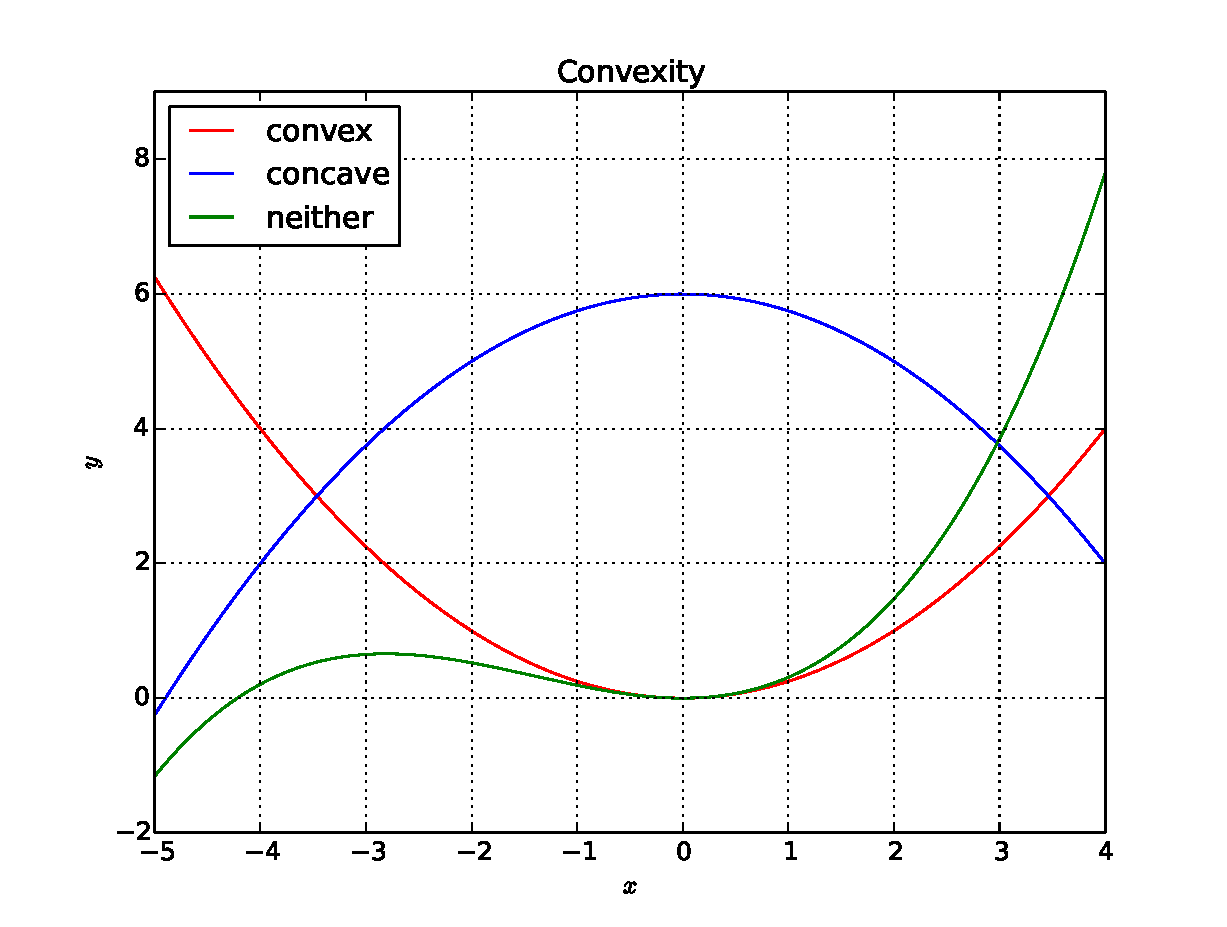
\includegraphics[width=0.8\linewidth]{fig/convexity.pdf}
    \caption{An illustration of convex and concave functions, along with
    an example of a funciton which is neither concave nor convex.}
    \label{fig:convex}
\end{figure}

A natural generalization of this idea is to say a function $f : \RR^n \mapsto \RR$ is
convex if $\nabla^2 f \succeq 0$ and $f$ is concave if $\nabla^2 f \preceq 0$. That is
to say our generalized version of the second derivative is our generalized version of
positive. Similarly, if $\nabla^2 f \preceq 0$ for all inputs $\xx$ then $f$ is concave.
This will come up a lot.

\subsection{Gradients and Hessians of Quadratic and Linear Functions}

These functions are relatively simple but we will use them \textit{a lot}.\\
Suppose we have $\xx,\bb\in\RR^n$ and a function $f(\xx) = \bb^\T\xx$.
Then
\[
    f(\xx) = \sum_{i=1}^n \bb_i\xx_i,
\]
and
\[
    \frac{\partial f}{\partial \xx_k} = \frac{\partial}{\partial \xx_k} \sum_{i=1}^n \bb_i\xx_i = b_k.
\]
Thus the gradient $\nabla f = \nabla \bb^\T\xx = \bb$. In the single variable case
we have the familiar $\frac{d}{dx}(ax) = a$. It follows immediately because $\nabla^2 f
= \nabla (\nabla f)^\T$ that $\nabla^2 \bb^\T\xx = 0$.\\

Suppose we have the quadratic function $f(\xx) = \xx^\T A\xx$ where $A\in\SS^n$. Recall
\[
    f(\xx) = \sum_{i=1}^n\sum_{j=1}^n A_{ij}\xx_i\xx_j.
\]
There will be $n$ terms with $\xx_k$ in them, so
\[
    \frac{\partial f}{\partial \xx_k} = \frac{\partial}{\partial \xx_k} \sum_{i=1}^n\sum_{j=1}^n A_{ij}\xx_i\xx_j = 2\sum_{i=1}^nA_{ki}\xx_i = 2A_{k:}\xx
\]
Thus we have the gradient $\nabla f = \nabla \xx^\T A\xx = 2A\xx$. This should be reminiscent
of the single variable case $\frac{d}{dx}(ax^2) = 2ax$. Now we look for the Hessian of the
same quadratic $f$. Taking partials, it follows that
\[
    \frac{\partial^2 f}{\partial \xx_k\partial \xx_l} = \frac{\partial}{\partial \xx_k}\left[ \frac{\partial f}{\partial \xx_l} \right] = \frac{\partial}{\partial \xx_k} 2A_{k:}\xx = 2A_{kl}.
\]
Thus the Hessian $\nabla^2 f = \nabla^2 \xx^\T A\xx = 2A$, which should be reminiscent of
as single variable cave $\frac{d^2}{dx^2}(ax^2) = 2a$.\\

It should then be obvious, because scaling preserves convexity, that any quadratic function
\[
    f(\xx) = \xx^\T A\xx + \bb^\T\xx + \cc
\]
is convex if and only if $A \succeq 0$ and concave if and only if $A \preceq 0$. In the case
that $A=O$ (the null matrix containing all zeroes) we have shown that a linear function
$f(\xx) = \bb^\T\xx + \cc$ is both concave and convex, just as in the single variable case!\\

To recap:
\begin{figure}[htpb]
    \centering
    \begin{tabular}{c|c|c}
        $f$ & $\nabla f$ & $\nabla^2 f$\\
        $\bb^\T\xx$ & $\bb$ & $0$\\
        $\xx^\T A\xx$ & $2A\xx$ & $2A$
    \end{tabular}
    \caption{Gradients and Hessians of very common functions
    involving linear operations.}
    \label{table:derivs}
\end{figure}

\subsubsection{Taylor Expansions: $f(\xx) \approx f(\aa) + \nabla f(\aa)^\T (\xx-\aa) + \frac{1}{2}(\xx-\aa)^\T \nabla^2 f (\xx-\aa)$}

You should already be familiar with Taylor's Theorem for a single variable function
$f : \RR \mapsto \RR$, where, about some point $a$
\[
    f(x) \approx f(a) + f'(a)(x-a) + \frac{f''(a)}{2}(x-a)^2 + \dots.
\]

We can extend this (without proof) to multiple variable functions
$f : \RR^n \mapsto \RR$ up to a quadratic approximation (you would need
to invoke tensors for higher orders: ew!) as
\[
    f(\xx) \approx f(\aa) + \nabla f^\T(\xx-\aa) + \frac{1}{2}(\xx-\aa)^\T \nabla^2 f (\xx-\aa).
\]
It follows immediately that if $f$ is convex or concave, the quadratic
Taylor approximation of $f$ is simiarly convex or concave, respectively.
This will be usefull in the context of the Newton-Raphson method for
convex optimization.

\subsection{Least Squares}

Now let's re-derive the closed form expression for fitting a line
to data. Suppose we are given matrices $A\in\RR^{m\times n}$ (where
$A$ is full rank) and a vector $\bb\in\RR^m$. We want to find a vector
$\xx\in\RR^n$ such that $A\xx=\bb$, but $\bb$ may be outside the
columnspace of $A$ (because $A$ is tall). Therefore we try to find
$\xx$ so that we minimize the $\ell-2$ distance from $A\xx$ to $\bb$.
That is,
\[
    \text{minimize: } f(\xx) = ||A\xx - \bb||_2^2 = (A\xx - \bb)^\T(A\xx-\bb) = \xx^\T A^\T A\xx - 2\bb^\T A\xx + \bb^\T\bb.
\]
At the minimum (because this problem is unconstrained) $\nabla f = 0$, so
\[
    \nabla \left(\xx^\T A^\T A\xx - 2\bb^\T A\xx + \bb^\T\bb\right) = 2A^\T A\xx - 2A^\T \bb = 0,
\]
so we see that
\[
    \xx = (A^\T A)^{-1}A^\T\bb,
\]
as desired.

\subsection{Eigenvalues as Optimization}

Now we will consider an optimization problem that we will see when
discussing Principal Component Analysis, which will lead directly
to eigenvalues and eigenvectors. Consider the following problem:
\begin{align*}
    \text{maximize: } & \xx^\T A\xx\\
    \text{subj. to: } & ||\xx||_2 = 1\\
\end{align*}
where $A\in\SS^n$.
First note that the constraint is the same as $||\xx||_2^2 = \xx^\T\xx = 1$.
We can form the Lagrangian of this problem (don't worry if you haven't seen this we
will see it much more in the future) as
\[
    \mathcal{L}(x,\lambda) = \xx^\T A\xx - \lambda (\xx^\T\xx - 1).
\]
at the optimal value it can be shown as part of the KKT conditions that
$\nabla_\xx \mathcal{L} = \0$, so
\[
    \nabla_\xx \mathcal{L} = 2A\xx - 2\lambda\xx = 0,
\]
so any optimum (maximum or minimum) must satisfy
\[
    A\xx = \lambda\xx,
\]
an eigenvalue-eigenvector pair! It can be shown that the largest eigenvalue
corresponds to the maximum of $\xx^\T A\xx$ and the smallest eigenvalue corresponds
to the minimum of $\xx^\T A\xx$.

\end{document}
